\documentclass[a4paper]{article}

%% Language and font encodings
\usepackage[english]{babel}
\usepackage[utf8x]{inputenc}
\usepackage[T1]{fontenc}

%% Sets page size and margins
\usepackage[a4paper,top=3cm,bottom=2cm,left=3cm,right=3cm,marginparwidth=1.75cm]{geometry}

%% Useful packages
\usepackage{amsmath}
\usepackage{graphicx}
\usepackage{caption}
\usepackage{subcaption}
\usepackage[colorinlistoftodos]{todonotes}
\usepackage[colorlinks=true, allcolors=blue]{hyperref}

\title{Reporte de Actividad 8: Oscilador Van der Pol}
\author{Jesús Antonio González Espinosa \\ \\ Física Computacional 1}
\date{Viernes, 13 de Marzo del 2018}

\begin{document}
\maketitle
\section{Introducción - Antecedentes}

Durante la actividad número 8 del curso, hemos estudiado el oscilador de Van der Pol. El tema, como en las últimas dos prácticas, sigue relacionado con el trabajo de ecuaciones diferenciales no lineales. 

Como lo dice el nombre, esta oscilación fue propuesta por Balthasar Van der Pol que vivió de 1889 a 1959, fue un físico holandés, que dedico su vida al estudio de la propagación de radio ondas, la teoría de los circuitos eléctricos y física matemáticas. Además de la oscilación de Van der Pol, hay un meteorito que también lleva su nombre. Entre sus sucesos y premios destacados se encuentra el recibimiento de un premio por el Instituto de Radio Ingenieros, y la entrada a la Real Academia de Ciencia y Artes de los Países Bajos. 

Van der Pol, al estar trabajando, encontró oscilaciones estables, que llamó oscilaciones de relajación. En 1927 publicó la información de su descubrimiento, que más tarde sería reconocido por la Teoría del Caos, como un fenómeno caótico. 

Durante el transcurso de la actividad se ha de mostrar varios ejemplos de resultados de la ecuación de Van der Pol. 

\section{Modelo Van der Pol}

El oscilador de Van der Pol no es conservativo, al incluir amortiguamiento. Está dado por la siguiente ecuación diferencial de segundo orden:
\begin{center}
$\frac{d^2x}{dt^2} - \mu (1 - x^2)\frac{dx}{dt} + x = 0$
\end{center}

Donde x describe la posición y t el tiempo. Siendo $\mu$ el coeficiente de fricción.  

\subsection{Forma Bidimensional}
A partir del teorema de Liénard esta ecuación se puede separar de forma dos dimensional para que resulten dos ecuaciones diferenciales de primer orden:
\begin{center}
$\dot{x} = \mu (x - \frac{1}{3} x^3 - y)$

$\dot{y} = \frac{1}{\mu} x$
\end{center}

También existe otra forma comúnmente utilizada. Ésta fue la que se usó para la actividad. 
\begin{center}
$\dot{x} = y$

$\dot{y} = \mu(1 - x^2)y - x$
\end{center}

\subsection{Resultados del Oscilador no Forzado}
A partir de la ecuación sin forzamiento, se pueden obtener resultados interesantes:
\begin{itemize}
\item Si el coeficiente de amortiguamiento es 0, la ecuación resulta en la forma de un oscilador armónico simple, donde siempre hay conservación de la energía.
\item Si el coeficiente de amortiguamiento es mayor que 0, el sistema va a entrar a un ciclo limite. Cerca del origen, el sistema estará inestable y lejos del origen estará amortiguado. 
\item Algo importante de mencionar es que el oscilador Van der Pol no tiene una solución analítica exacta. 
\end{itemize}

\subsection{Hamiltoniano para el Oscilador Van der Pol}
Se puede escribir un formalismo hamiltoniano independiente del tiempo para el oscilador Van der Pol aumentándolo a un sistema dinámico autónomo tetradimensional usando una ecuación diferencial no lineal de segundo orden auxiliar de la siguiente manera:
\begin{center}
$\ddot{x} - \mu(1 - x^2)\dot{x} + x = 0$
$\ddot{y} + \mu(1 - x^2)\dot{y} +y = 0$
\end{center}

La dinámica del oscilador original Van der Pol no se ve afectada por el acoplamiento unidireccional entre las evoluciones temporales de las variables $x$ y $y$. Se puede demostrar que una Hamiltoniana $H$ para este sistema de ecuaciones es:

\begin{center}
$H(x,y,p_x,p_y) = p_xp_y + xy - \mu(1 - x^2)yp_y$
\end{center}

donde $p_x$ y $p_y$ son los momentos conjugados correspondientes a $x$ y $y$ respectivamente.

\subsection{Oscilador Van der Pol Forzado}

El oscilador Van der Pol forzado es la ecuación original con una función de conducción, resultando en:

\begin{center}
$\frac{d^2x}{dt^2} - \mu(1 - x^2)\frac{dx}{dt} + x - ASin(\omega*t) = 0$
\end{center}

donde $A$ es la amplitud de la función de onda y $\omega$ su velocidad angular. 

\section{Exploración de Soluciones}
En esta sección se van a mostrar diferentes gráficas de la fase, donde se modifican los valores iniciales con el fin de demostrar que a pesar de las variaciones en los datos, la oscilación de Van der Pol va a llegar a resultados repetitivos muy parecidos entre ellos.

Para esto, en Python se utilizó una combinación de los códigos utilizados en las actividades 6 y 7, junto con pedazos nuevos obtenidos del SciPy Cookbook del artículo de Lotka-Volterra.

Primero se declaran las ecuaciones:
\begin{figure}[ht!]
 \centering
  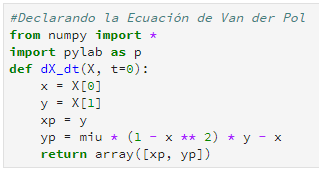
\includegraphics[width=0.5\textwidth]{Codigo1.PNG}
\end{figure}

\pagebreak

A partir de estas, se declaran las condiciones iniciales:
Primero se declaran las ecuaciones:
\begin{figure}[ht!]
 \centering
  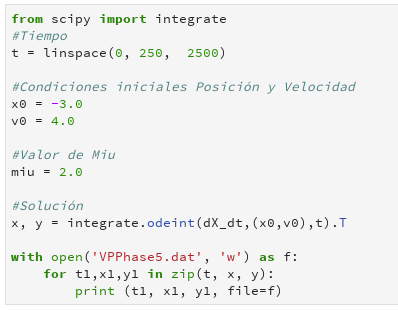
\includegraphics[width=0.5\textwidth]{CodigoEx1.png}
\end{figure}

Como se puede ver en la imagen, las condiciones iniciales son:
\begin{itemize}
\item $\mu = 2$
\item $x_0 = -3$
\item $v_0 = 4$
\item tiempo de 0 a 250 segundos
\end{itemize}

La gráfica resultante es:

\begin{figure}[ht!]
 \centering
  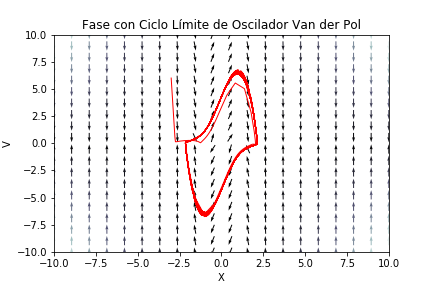
\includegraphics[width=0.8\textwidth]{VP_Ex1.png}
\end{figure}

A partir de esto, se hicieron otras modificaciones a las condiciones iniciales, creando las siguientes gráficas (se mantuvo el mismo tiempo en todos las recreaciones):

\pagebreak

\begin{figure}[ht!]
\begin{subfigure}{0.5\textwidth}
  \centering
  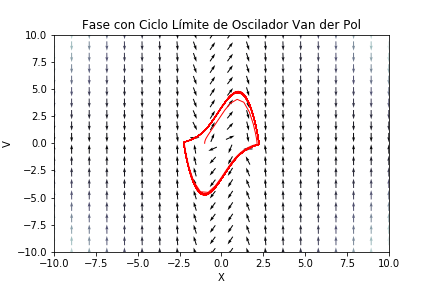
\includegraphics[width=\linewidth]{VP_Ex2.png}
   \caption{$\mu = 2, x_0 = -1, v_0 = 0$}
\end{subfigure}
\begin{subfigure}{0.5\textwidth}
  \centering
  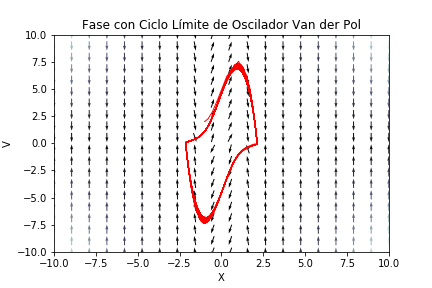
\includegraphics[width=\linewidth]{VP_Ex3.png}
  \caption{$\mu = 4, x_0 = -1, v_0 = 2$}
\end{subfigure}
\begin{subfigure}{0.5\textwidth}
  \centering
  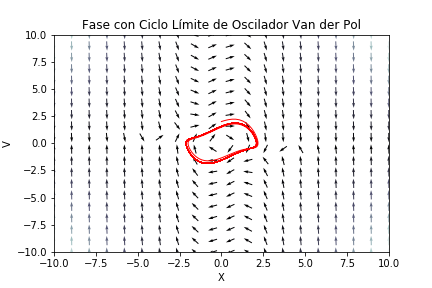
\includegraphics[width=\linewidth]{VP_Ex4.png}
  \caption{$\mu = 0.5, x_0 = 0, v_0 = 2$}
\end{subfigure}
\begin{subfigure}{0.5\textwidth}
  \centering
  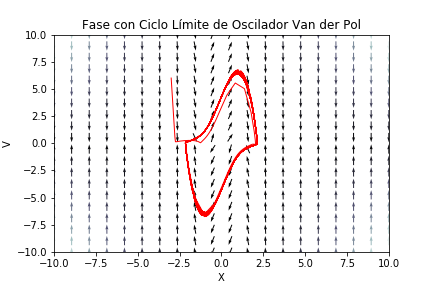
\includegraphics[width=\linewidth]{VP_Ex5.png}
  \caption{P$\mu = 3.5, x_0 = -3, v_0 = 6$}
\end{subfigure}
\end{figure}

En todos podemos notar que al pasar el tiempo, el ciclo límite es muy parecido en todos, a pesar de sus condiciones iniciales.


\section{Resultados}
Siguiendo la misma idea y ecuación declarada en la sección anterior, ahora nos enfocamos más en una recreación exacta de las gráficas del artículo de Wikipedia más que en explorar los resultados.

Para la primera, al observar las gráficas podemos obtener las condiciones iniciales de los retratos de las fases. Algo importante es que todos deben mantener el mismo valor de $\mu$ para que resulte igual. Se guardaron las soluciones en archivos resultados para posteriormente graficarlos. El código resultó de la siguiente manera:
\begin{figure}[ht!]
 \centering
  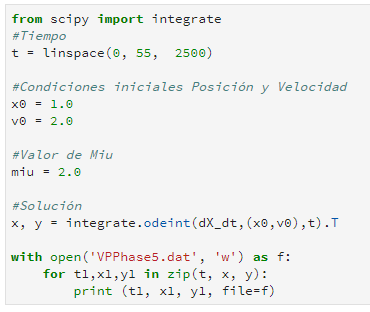
\includegraphics[width=0.6\textwidth]{Codigo2.PNG}
\end{figure}
\pagebreak
\begin{figure}[ht!]
 \centering
  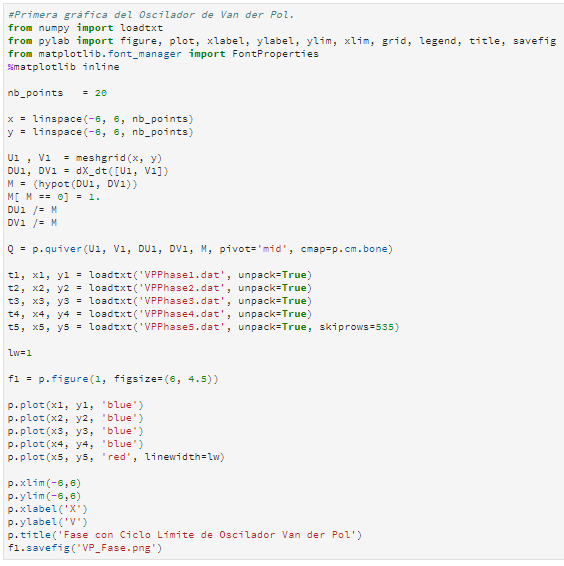
\includegraphics[width=0.6\textwidth]{Codigo3.PNG}
\end{figure}

En la primer imagen fue el segmento de código que ayudó a guardar las 4 soluciones diferentes a partir de las condiciones iniciales de Posición y Velocidad de cada oscilación. En la siguiente imagen podemos ver el código que sirvió para graficar cada fase y presentar el campo vectorial.

\begin{figure}[ht!]
 \centering
  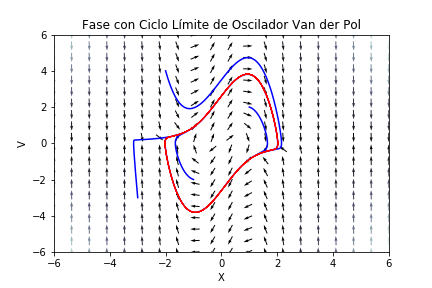
\includegraphics[width=0.8\textwidth]{VP_Fase.png}
\end{figure}

En la cual se graficaron los 4 fases, donde se muestra que todas llegan al mismo ciclo límite. En todas se uso el valor de $\mu = 2$.
\bigskip

Para la siguiente gráfica se mantuvo una idea parecida, pero ahora lo que varía fue el valor del amortiguamiento, pero no los valores iniciales. Se generaron varios archivos que guardan los soluciones de la ecuación con los diferentes valores de $\mu$. Por lo tanto, el código es casi exactamente igual al de la gráfica uno, solo que creando 10 archivos, cada uno con los diferentes valores de $\mu$. La gráfica resultante fue:

\pagebreak

\begin{figure}[h!]
 \centering
  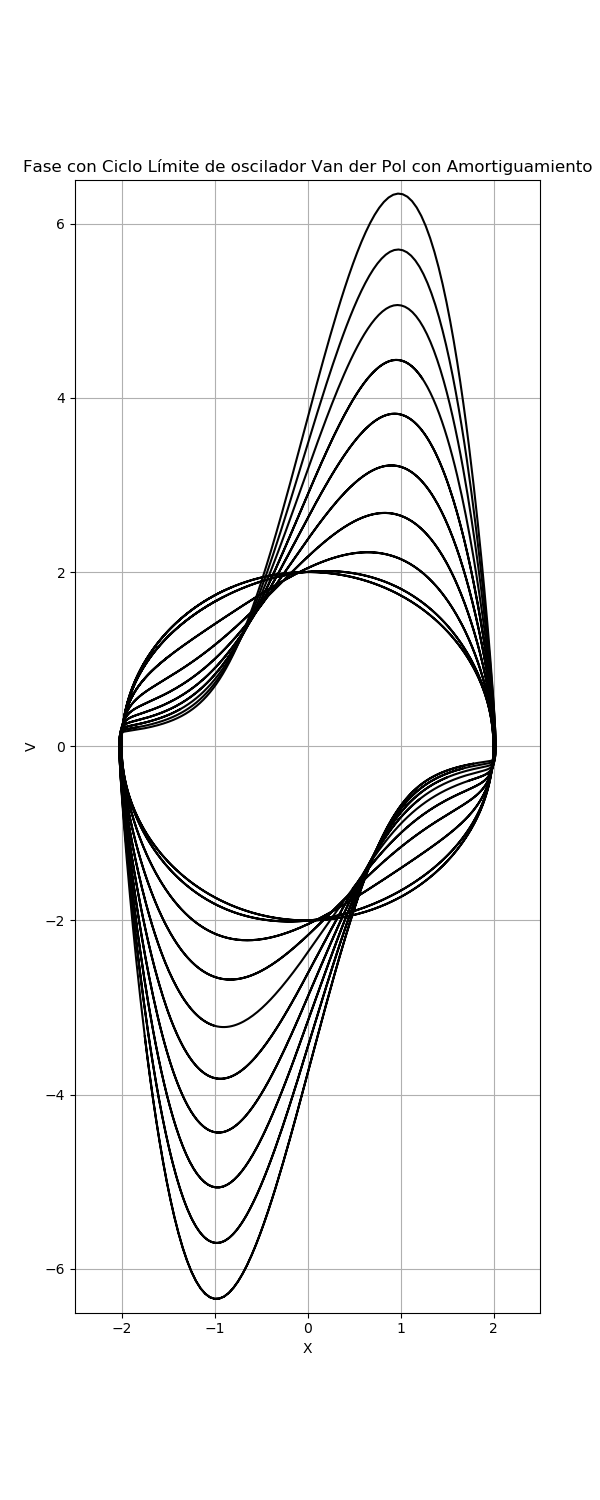
\includegraphics[width=0.5\textwidth]{VP_Miu.png}
\end{figure}

Donde el valor de $\mu$ más alto corresponde a la fase más alta y mediante va disminuyendo, en la gráfica también lo hace. Los valores de $\mu$ son: $4.0$ para el más alto, y descendiendo con $3.5, 3.0, 2.5, 2.0, 1.5, 1.0, 0.5, 0.1$, hasta el valor más pequeño, $0.01$ que corresponde a la fase más estrecho. 

\bigskip


Para la tercera gráfica, el código resulta más sencillo, ya que ésta muestra la variación de la posición del oscilador con respecto al tiempo. Además te da el valor del amortiguamiento $\mu$ y además se puede observar el tiempo que dura en oscilación, así como su posición inicial. El código resulta así:

\begin{figure}[ht!]
 \centering
  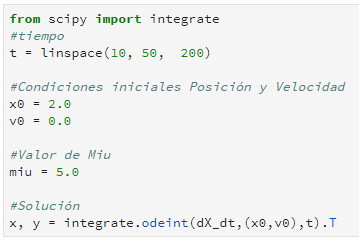
\includegraphics[width=0.6\textwidth]{Codigo6.PNG}
\end{figure}
\pagebreak
\begin{figure}[ht!]
 \centering
  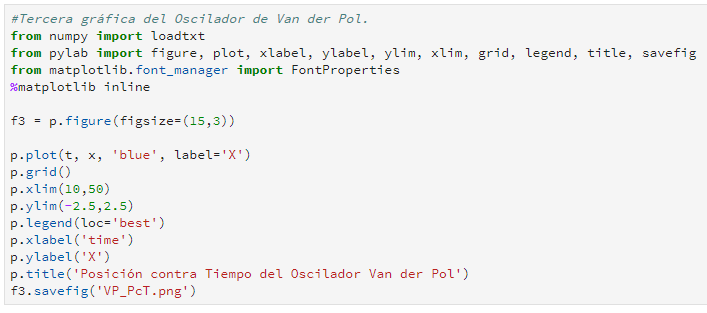
\includegraphics[width=0.6\textwidth]{Codigo7.PNG}
\end{figure}

Que genera la gráfica:

\begin{figure}[ht!]
 \centering
  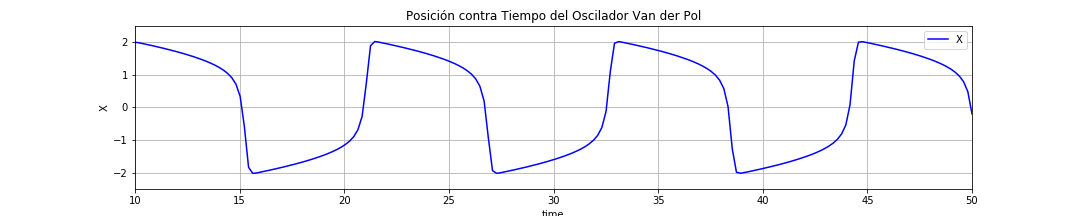
\includegraphics[width=\textwidth]{VP_PcT.png}
\end{figure}

Donde podemos ver el comportamiento de la posición con respecto al tiempo. 

\bigskip

Para la última gráfica, se repite el mismo proceso que la gráfica anterior, pero esta vez la ecuación muestra un comportamiento de forzamiento, por lo que tenemos que modificar el código para agregarle tal forzamiento a la ecuación de Van der Pol. Esta vez aparecen los parámetros de amplitud y velocidad angular, por lo que también se agregan al código. Los valores de tales parámetros aparecen en la imagen del artículo, junto con el valor de $\mu$, y de nuevo podemos ver el tiempo y la conidición inicial de posición en la imagen. El código para la gráfica es de la siguiente manera:

\begin{figure}[ht!]
 \centering
  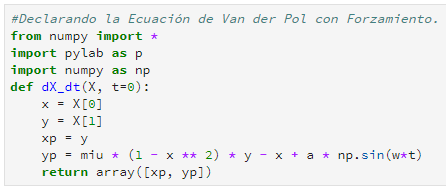
\includegraphics[width=0.6\textwidth]{Codigo8.PNG}
\end{figure}
\pagebreak
\begin{figure}[ht!]
 \centering
  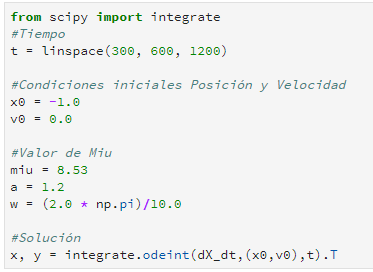
\includegraphics[width=0.6\textwidth]{Codigo9.PNG}
\end{figure}
\begin{figure}[ht!]
 \centering
  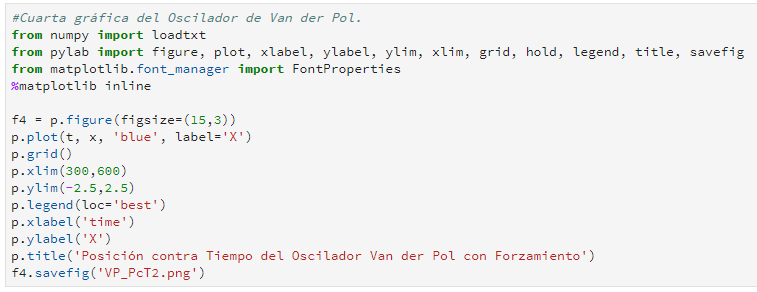
\includegraphics[width=0.6\textwidth]{Codigo10.PNG}
\end{figure}

En donde en la primer imagen podemos ver como se agrega el forzamiento a la ecuación de Van der Pol; en la segunda vemos los parámetros y sus condiciones iniciales; y en la tercera vemos como se graficaron los datos. La cual resultó así:

\begin{figure}[ht!]
 \centering
  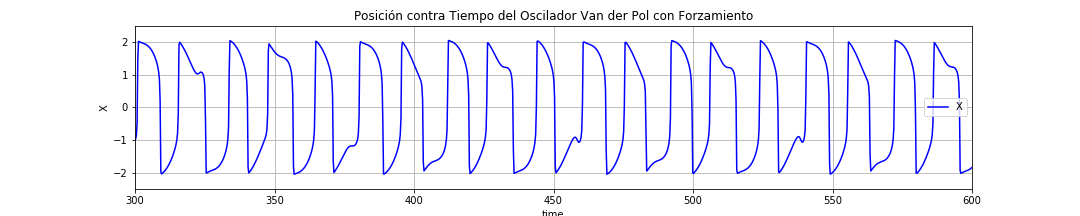
\includegraphics[width=\textwidth]{VP_PcT2.png}
\end{figure}

Donde se puede ver el forzamiento que afecta a la posición con respecto al tiempo.

\bigskip

\section{Conclusión}
El estudio del oscilador de Van der Pol ha sido interesante, se han visto comportamientos extremos y muy sensibles a pequeñas modificaciones a las condiciones iniciales, especialmente por el coeficiente de amortiguamiento, justo como se había previsto. Por otra parte, el haber conocido sobre la Teoría del Caos, al ser este un gran ejemplo.

A pesar de haber sido relacionado con el tema de las dos prácticas pasadas, al trabajar con esta actividad, se creo un ambiente muy diferente, ya que hubo un mayor grado de dificultad en las necesidades para poder reproducir las gráficas a partir del modelo de las ecuaciones; pero fue esa dificultad lo que a la vez lo hizo un reto más entretenido. 

\pagebreak

\section{Bilbiografía}
\begin{itemize}
\item Wikipedia (2018) Van der Pol oscillator. Recuperado el 09 de Abril del 2018 desde 

https://en.wikipedia.org/wiki/Van\_der\_Pol\_oscillator
\item Wikipedia (2017) Balthasar van der Pol. Recuperado el 10 de Abril del 2018 desde 

https://en.wikipedia.org/wiki/Balthasar\_van\_der\_Pol
\item SciPy Cookbook (2017) Matplotlib: Lotka Volterra Tutorial. Recuperado el 05 de Abril del 2018 desde

http://scipy-cookbook.readthedocs.io/items/LoktaVolterraTutorial.html
\end{itemize}

\section{Apéndice}
\begin{enumerate}
\item \textbf{Este ejercicio pareciera similar al desarrollado en las actividades 6 y 7. ¿Qué aprendiste nuevo?}

Aunque fue muy similar en cuanto a la solución de los sistemas; de esta actividad aprendí sobre el modelo de Van der Pol, un poco de la Teoría del Caos, y cómo agregar campos vectoriales a las gráficas. En otras palabras, un poco de todo de los temas necesarios para completar la actividad.

\item \textbf{Has escuchado ya hablar de caos. ¿Por qué sería importante estudiar este oscilador?}

Sí, lo he escuchado, pero muy por encima, antes de esta actividad no lo conocía lo suficiente como para decir que estaba familiarizado con el concepto. Es importante estudiar este oscilador porque presenta resultados muy interesantes, que como ya vimos, van relacionados con el caos.

\item \textbf{¿Qué mejorarías en esta actividad?}

No creo que haya algo necesario para mejorar, ya que aunque la actividad fue un poco complicada, el tiempo fue suficiente para entender los conceptos necesarios y trabajarlos.

\item \textbf{¿Algún comentario adicional antes de dejar de trabajar en Jupyter con Python?}

Trabajar en Jupyter con Python ha sido una experiencia muy entretenida y positiva, ha sido más agradable que Fortran, que es el otro lenguaje que conozco, ya que me aportó un entorno que sentí más cómodo. 

\item \textbf{Cerramos la parte de trabajo con Python ¿Que te ha parecido?}

Ha sido interesante porque, aunque nunca desarrollamos un código totalmente desde cero nosotros mismos, entender los códigos aportados por el profesor se podría decir que fue sencillo. 
\end{enumerate}

\end{document}